\chapter{Prototype Peer-to-Peer Web Access over Bluetooth}
\label{chapter:work}

In this chapter the developed peer-to-peer communication prototype will be analysed. This explanation will address the decisions about the technology and protocols to use as well as the architecture and workflow of the application.

It will begin with a brief summary of the steps taken to reach the developed application's architecture and functionality. After the overall application's objectives and high-level architecture is described, a section on the lower-level architecture and processes of the application will be presented. Finally, there will be a section describing the conclusions on the developed work, from its limitations to the possible future work.

\section{Design Choices}

This section will provide the explanation and justification of the choices made for the application type, ad hoc communication technology, ad hoc network topology and ad hoc routing protocol.

\subsection{Application Type}

The choice of the target application was mainly based on the innovation criterium. For this purpose, an investigation was made on already existing peer-to-peer applications, see Section \ref{sec:apps}. Most of the existing applications are designed to support text messaging with much of the developed work focusing on recreating popular applications, such as Messenger and WhatsApp, using a peer-to-peer network to route the messages to their destinations. Beaconing and geolocation messages are also not completely innovative, since applications such as Uepaa!, see Subsection \ref{subsec:uepaa}, already implement peer-to-peer applications where these types of messages are exchanged. Given this reasoning it was considered that the most innovative application type would be web browsing, supporting a multi-hop hot spot in an ad hoc network.

\subsection{Ad Hoc Communication Technology}

The choice of ad hoc network technology was another important step. The first and most obvious choice would be to use Wi-Fi Direct in both advertising and communication between devices, since this technology offers the best features to transfer files around \textit{1KB}, in both range and data rate of transmission. However, during the development it proved to be impossible to continue with this approach, as Wi-Fi Direct's current Android implementation does not allow for devices to transfer files without active user participation, also mentioned in \cite{bwmesh}.

Given this drawback a shift to Bluetooth was made, and a hybrid version of the application was created, where the advertisement would be done via Wi-Fi Direct and the actual transfer of the web pages would be made via Bluetooth. This method also proved to be infeasible, due to security issues, since the the devices would have to display their Bluetooth MAC addresses in their Bluetooth name, making them much more vulnerable to possible attacks.

The advertisement was also a topic of debate. Two possibilities were presented: to use simple Bluetooth connections to advertise to each peer or to use \gls{BLE} beacons as an advertisement method. The first method is slower, since the advertising device needs to create a connection with each discovered peer, in order to transmit its advertisement. The second method would offer a better advertisement mechanism, since it is faster and consumes less resources than the traditional Bluetooth connections (see Subsection \ref{subsection:bt}), but it gives every device the ability to capture the advertisement, bringing some security issues.

The beacon advertisement is a tempting mechanism to implement, given all its advantages. It comprises two components: transmission and ranging. Transmission occurs when a device wants to issue an advertisement to a certain region\footnote{A beacon region is the physical space reached by the advertisement.}. Ranging is the act of listening to beacon transmissions in a certain region. During the implementation of these two components it was possible to verify that the current Android implementations - tested with Android versions 6.0 and 7.0 - are not able to reproduce \gls{BLE}'s transmission mechanism, being only able to use the ranging.

Given these facts, the application was developed using simple Bluetooth connections for both advertisement of the devices and data transfer. Although this is not the best technology for communication in an ad hoc network, it is the only one that currently meets all the requirements for this work. In the end of this section, a brief discussion on the changes that need to be made to Wi-Fi Direct's implementation in Android will be presented, and why developers could benefit from these changes.

\subsection{Ad Hoc Routing Protocol}
\label{subsec:routprot}

The last step was to create/modify a routing algorithm to control the destination of each incoming message. The requirements are simple: the algorithm simply needs to save the next hop of the shortest path leading to a device with Internet connection.

\gls{DSDV} is a routing protocol used in ad hoc mobile networks. This protocol uses a routing table where it stores in each entry the destination, next hop, number of hops to reach the destination and a sequence number to avoid routing loops. The devices exchange full routing tables, creating a network where every device has total knowledge of the topology. However, \gls{DSDV} requires the exchange of routing tables and their regular updates, wasting bandwidth - see \cite{dsdv} for more information on \gls{DSDV}.

\gls{AODV} is also a known routing scheme used in ad hoc mobile networks. It establishes paths in a reactive way, \textit{i.e.} only when a device wants to retrieve a web page does this protocol search for a path in which to send the packet - see \cite{aodv} for the full specification of this scheme. This scheme is not the most reliable, since the requesting device should know beforehand if it is capable of reaching the Internet, otherwise users will uselessly experience long periods of path requesting and advertising every time they request a web page.

The proposed application does not have a specific destination as a goal, \textit{i.e.}, a device A does not want to transmit to B, it only wants to reach a node with network access with the minimum amount of hops. Hence, the sending device will have no need to know the elements of the routing path, other than the next hop node. Thus, in order to accommodate such requirements some modifications were made to \gls{DSDV}. Firstly, to reduce the signalling overhead used by \gls{DSDV}, the developed version will simply exchange the best next hop estimate of the current device. Secondly, instead of a periodic exchange of tables, devices will update their tables every time a new Advertisement message is received and they only exchange routing information when a new best path is received.

After a flexible period of time, each device erases its routing table and proceeds to restart the discovery and advertisement protocol - see Subsection \ref{subsec:disandadv}. This allows devices to adjust their routing tables to the network's changes, such as erasing routes that no longer are available and replacing them with newly created ones. The period is flexible and can be changed according the dynamics of the network.

The proposed protocol provides a loop-free path for every request, since every node only advertises the best hop distance estimate. The downfall is that the requests' paths are not flexible, \textit{i.e.}, a Request message is always sent through the best path and, if a link along that path is broken, the Request message is discarded. New paths are only established periodically, when a new round of advertisements is performed, as mentioned in the previous paragraph.

A different routing protocol could be deployed, one that has more flexibility, regarding the requests' paths. A possible approach could be to use a similar Advertisement message structure as the one used in \gls{DSDV}. The \gls{MAC} address of the advertisement creator would be added, as well as a sequence number. These new message fields would be used to assess if the received advertisement is newer than the previously received advertisement from that node, or was simply delayed. With this mechanism, it would be possible to establish several secondary path if the best path was inaccessible.

However, to establish such protocol, would add complexity and consume time resources during both the advertisement and web page exchange processes. Nevertheless, this option could be implemented, in an application for which reliability is more important than delay.

Since this work aims to to develop a peer-to-peer web access, the time of data exchange is crucial, as this application would be useless if the time to access the Internet is too big. Thus, the first, lighter routing protocol was implemented.

\section{Architecture}
\label{sec:architecture}

In this section the architectures of both framework and application are presented.

The developed framework and application's main structure are similar and consist of:

\begin{itemize}
	\item A routing algorithm that controls the destinations of the packets in each hop.
	\item A communication technology, \textit{e.g.} Bluetooth or Wi-Fi Direct, handler, for both discovering nearby devices and to establish communication sockets with peers.
	\item A set of functions capable of analysing incoming messages and deciding which is the next step to perform, in order to complete the requests/advertises.
	\item Finally, in the application, a user interface is necessary, where the incoming messages can be seen and analysed (for debug purposes), also providing a text area for the user to enter the requested data.
\end{itemize}

In Figure \ref{fig:appsandbox} an overview of the developed application is shown. It can be seen that there are two main parts of the application: the main activity and the \textit{BluetoothService}.

\begin{figure}[ht]
	\noindent\makebox[\textwidth]
	{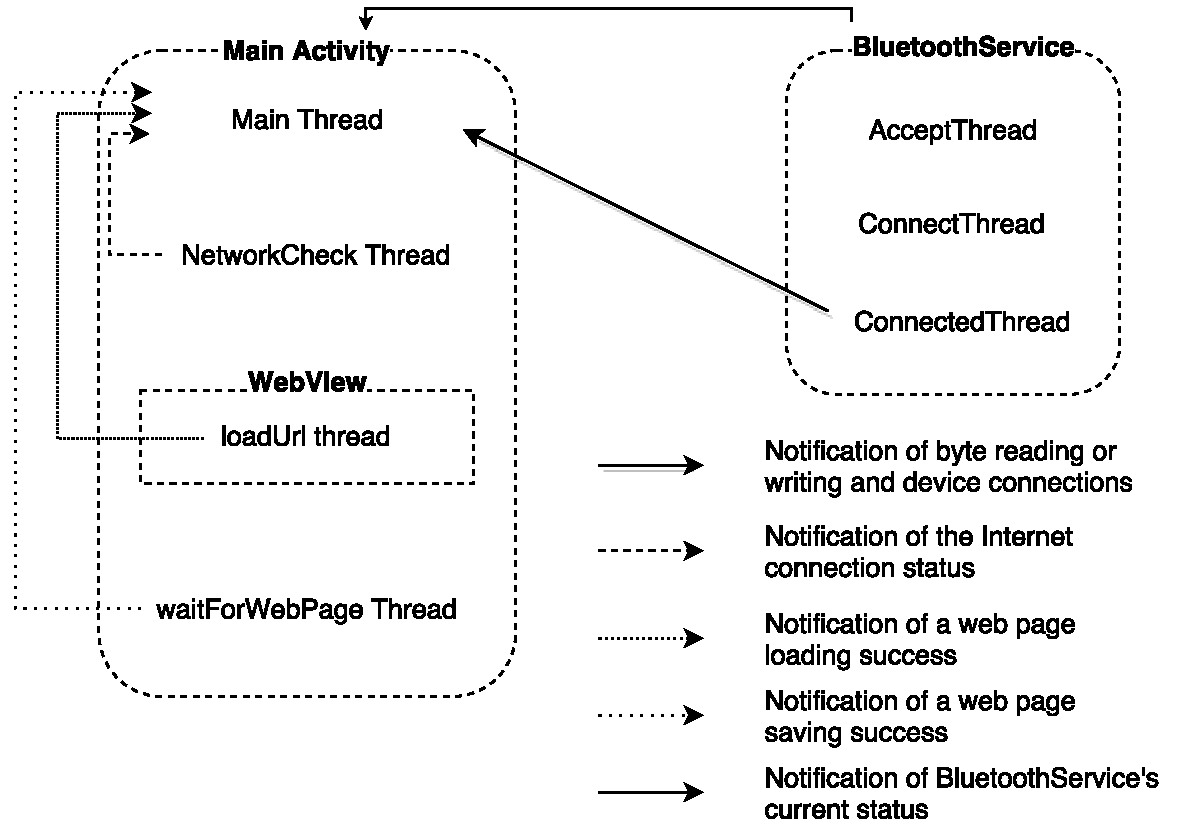
\includegraphics[width=1\textwidth]{images/app_sandbox.pdf}}
	\caption{\label{fig:appsandbox} Overview of the different parts of the application and the communication between the threads running in each part.}
\end{figure}

\begin{itemize}

\item The main activity is where most of the processing logic is executed, from the analysis of the received data to the management of the routing tables. It comprises four threads: the \textit{Main} thread seen by the user, also known as the user interface thread; the \textit{NetworkCheck} thread, used to perform the query regarding the Internet connection status of the device; the \textit{LoadUrl} thread, created when a \textit{WebView} object is used to show or download a web page; finally, the \textit{WaitForWebPage} Thread used to ensure the requested web page is successfully saved in the device.

\item The \textit{BluetoothService} is used to manage the Bluetooth connections between devices, it comprises three threads: the \textit{AcceptThread}, the \textit{ConnectThread} and the \textit{ConnectedThread}. Each of these threads will be explained in detail in the next subsection.

\end{itemize}

Inside the main activity the different threads communicate with each other, mainly to notify the \textit{Main} thread of a certain occurrence that may lead to a new set of actions. However, communication is also done between the main activity and the service, usually when the former needs to access the \textit{BluetoothService}'s current status.

\subsection{Bluetooth Connections}
\label{subsec:btconn}

In this subsection, the Bluetooth connections between devices and their possible stages will be described and analysed.

Since the communication technology is Bluetooth, the application must have a thread\footnote{Thread is a sequence of instructions managed independently, usually by a scheduler from the operating system. See \cite{threads} for more documentation on threads.} that handles the listening and acceptance of connections and the data transfer between devices. This corresponds to the \textit{BluetoothService.java} class. It creates and listens to insecure communication sockets, allowing devices to exchange data without user intervention.

The service has three different threads within it: a thread for the acceptance of incoming communications - \textit{AcceptThread}; a thread for the initial exchange of vital information before the connection - \textit{ConnectThread}; and a thread for the actual exchange of data between devices - \textit{ConnectedThread}. The connection of devices goes through each of these stages, allowing the \textit{Main} thread to get information on the connection status of the device at a given time.

There were two different approaches to the connections of devices: either the devices stayed connected as long as possible until a new connection was requested, or the devices stayed connected for the minimal amount of time for data to be transferred. The second approach was used, since it is the one that is more energy efficient, draining a lower amount of energy from the device batteries.

Bluetooth communication between devices is only allowed if both devices have matching "credentials", providing a minimum amount of security to prevent against possible attacks. An application specific name and \gls{UUID} represent the application, making it distinguishable from any other, since the \gls{UUID} of an application should not be repeated in any other.

To notify the \textit{Main} thread about what is being done by the \textit{BluetoothService}, a handler is created, acting as bridge between the two parts. It can be used for various actions, such as: retrieving the status of a connection, assessing if a device is ready to receive a file, \textit{etc.}

Bluetooth connections can be in one of four stages: listening, connecting, connected and not enabled. Each thread mentioned earlier is the implementation of a stage.

In the next subsections each stage will be explained in detail, providing a better understanding on how the connections are managed.

\subsubsection{Listening}
\label{subsubsec:listening}

A device is said to be in the listening stage when it has no ongoing connection but it is waiting for a new one initiated by another device. It is the "first" stage of the \textit{BluetoothService}, since every time the service is initiated, the device is moved to this stage.

In Figure \ref{fig:btreceiver} the flow diagram of the performed actions from the point of view of a device that is waiting for incoming connections is presented.

\begin{figure}[ht]
	\noindent\makebox[\textwidth]
	{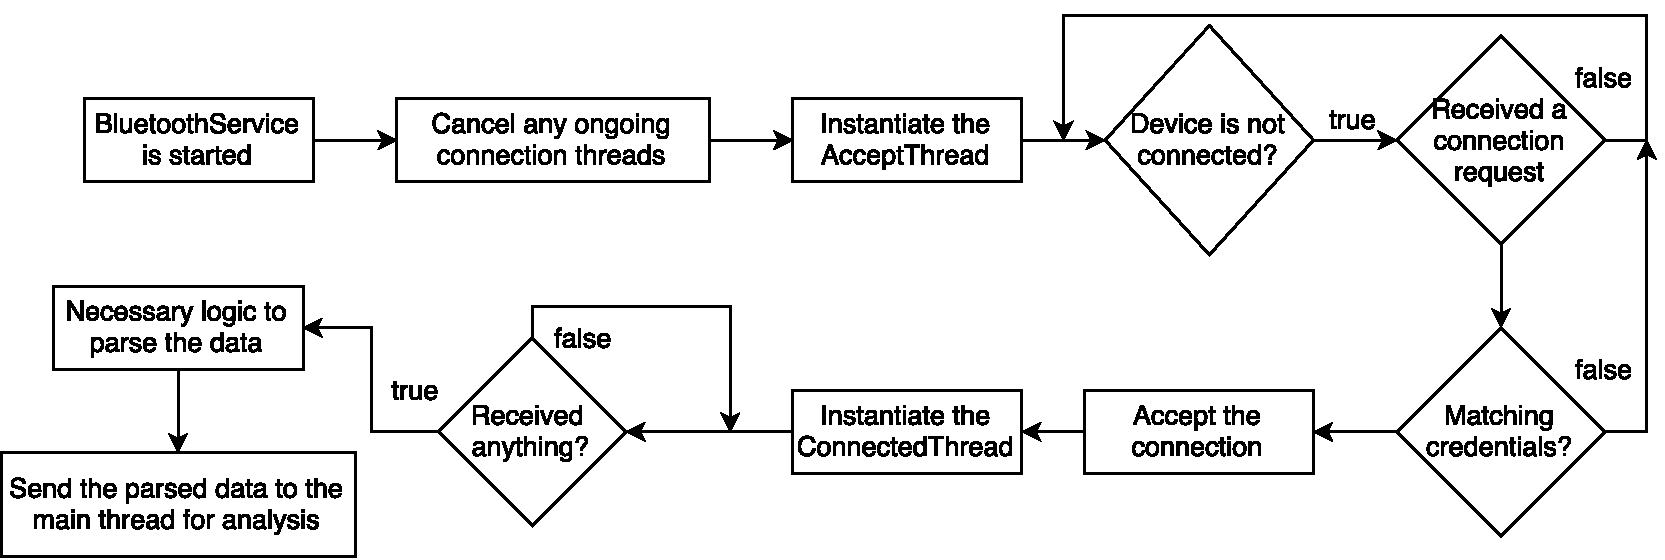
\includegraphics[width=1\textwidth]{images/btreceiver.pdf}}
	\caption{\label{fig:btreceiver} Flow diagram of the performed actions of a device listening for incoming connection requests.}
\end{figure}

As was said previously, each connection stage is associated with a thread class. The listening stage is associated with the \textit{AcceptThread}, which is instantiated every time the device enters this stage. The framework's connections have short durations and each time a new connection is performed, the service is restarted, entering the listening stage. Hence, it is imperative to assure there are no memory leaks or communication sockets left open. Thus, before the listening thread is instantiated, it is verified if any other Bluetooth connection threads are running, in which case they are shut down.

Once all the requirements for the instantiation of a new thread are met, a communication socket is created in which the device listens to incoming connection requests. To implement the listening mechanism, a loop is created whose purpose is to block the thread until a new connection is received, an error occurs or the user shuts down the application.

Whenever the device receives a new connection, it verifies the "credentials" sent in that connection request and compares them with the ones defined in its \textit{BluetoothService}. If they match, the connection is accepted.

Upon successfully accepting a connection, the method assesses the status of the newly formed connection and decides upon it. If everything goes as planned, the connection should now be in the connected stage. Once this migration between stages is concluded the instance of the listening thread is destroyed and a new connected thread is created.

\subsubsection{Connecting}
\label{subsubsec:connecting}

For a Bluetooth connection to be performed, at least two devices must exist, one of them acting as the connection initiator. In Figure \ref{fig:btrequester} the actions performed by a Bluetooth connection initiator during the connection establishment period are presented.

\begin{figure}[ht]
	\noindent\makebox[\textwidth]
	{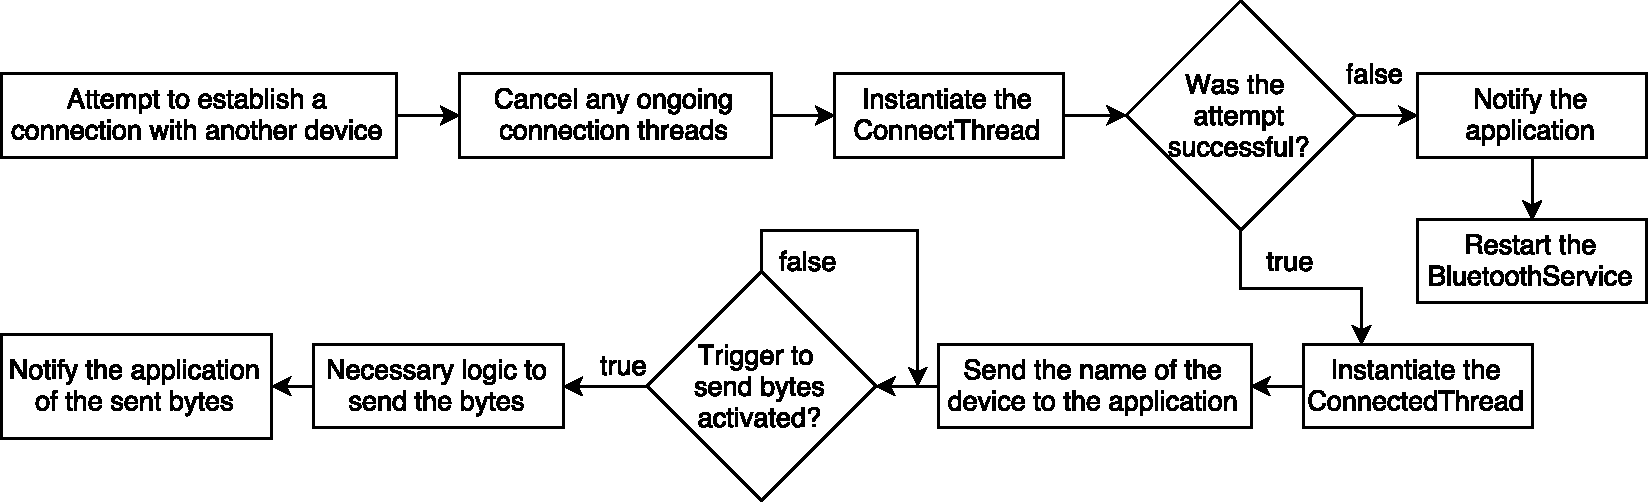
\includegraphics[width=1\textwidth]{images/btrequester.pdf}}
	\caption{\label{fig:btrequester} Flow diagram of a Bluetooth connection initiator's performed actions.}
\end{figure}

Similar to the listening thread initiation, the \textit{ConnectThread} is only instantiated after all the previous Bluetooth connection threads running in the device are shut down. Also, to avoid delays during the connection process, the Bluetooth discovery process is shut down. Only then can the initiator attempt to establish a connection with the desired device.

To identify the receiver of the connection request, the device needs to retrieve the \gls{MAC} address of its counterpart - this will be explained in Subsection \ref{subsec:disandadv}. Once this is attained, the connection initiator can attempt to create a communication socket between both devices, using the previously defined Bluetooth "credentials" and the receiver's \gls{MAC} address. If the \gls{MAC} address is valid and corresponds to a device within reach, the connection is requested successfully.

In case of failure due to the rejection of the connection from the receiver, a notification is sent to the \textit{Main} thread, notifying the connection was not successful and the service is restarted.

However, if the sent connection request is accepted by the receiver, the connection state is assessed and, if no interruptions or errors occur, the connection stage is moved to the connected stage, indicating both devices are able to send and receive bytes from their counterpart.

\subsubsection{Connected}
\label{subsubsec:connected}

When the connection reaches the connected state, both the connection initiator and the receiver devices are linked through a Bluetooth communication socket. To start the receiving and transmitting mechanisms, a \textit{ConnectedThread} is created, after all ongoing threads are cancelled to avoid conflicts between communications or memory leaks. To notify the \textit{Main} thread about the connection success, the service sends the counterpart's Bluetooth identifier, \textit{i.e.} its Bluetooth name, to the \textit{Main} thread.

To understand how data is transferred between the two connected devices it is necessary to explain two different mechanisms: the writing of data and the reading of data. By creating a socket linking both devices, two data streams are also created implicitly, where one provides a stream to write data into the socket and the other provides a stream to read data from the socket - see Figure \ref{fig:inoutstreams}. Both writing and reading data is in the form of byte arrays that can be afterwards manipulated into the desired format.

\begin{figure}[ht]
	\noindent\makebox[\textwidth]
	{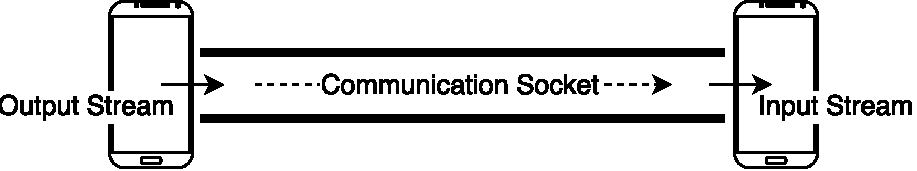
\includegraphics[width=0.8\textwidth]{images/inoutstreams.pdf}}
	\caption{\label{fig:inoutstreams} Communication channel with input and output streams.}
\end{figure}

Writing bytes into the socket is done through an output stream, name given to the part of the stream that handles the writing. For any data format, the principle is the same: to convert the data into a byte array that will be sent through the stream. It is important to note that the channel has a limited size buffer shrinking the arrays' size, thus if the data to be exchanged has a large amount of bytes, it is wise to perform segmentation. The writing process is asynchronous, since it is only executed at a certain time following a certain trigger, \textit{e.g.} user input. It is possible to notify the \textit{Main} thread about the sent bytes in case they are relevant to other processes, \textit{e.g.} notifying that a text message was sent and prepare to receive/send an image.

Reading data from the socket is done through an input stream. Since the output stream only writes byte arrays into the socket, the input stream will only read byte arrays. This property burdens the developer with the task of parsing the received bytes, \textit{i.e.} identifying them and then converting them into their original data type. Also, as mentioned before, the communication socket has a limited size buffer, thus it is also the developer's responsibility to perform segmentation and reassembly of the sent data.

In Figures \ref{fig:btconnectedr} and \ref{fig:btconnectedw}, the actions performed to read and write data from and to a Bluetooth communication socket are shown, respectively.

\begin{figure}[ht]
	\noindent\makebox[\textwidth]
	{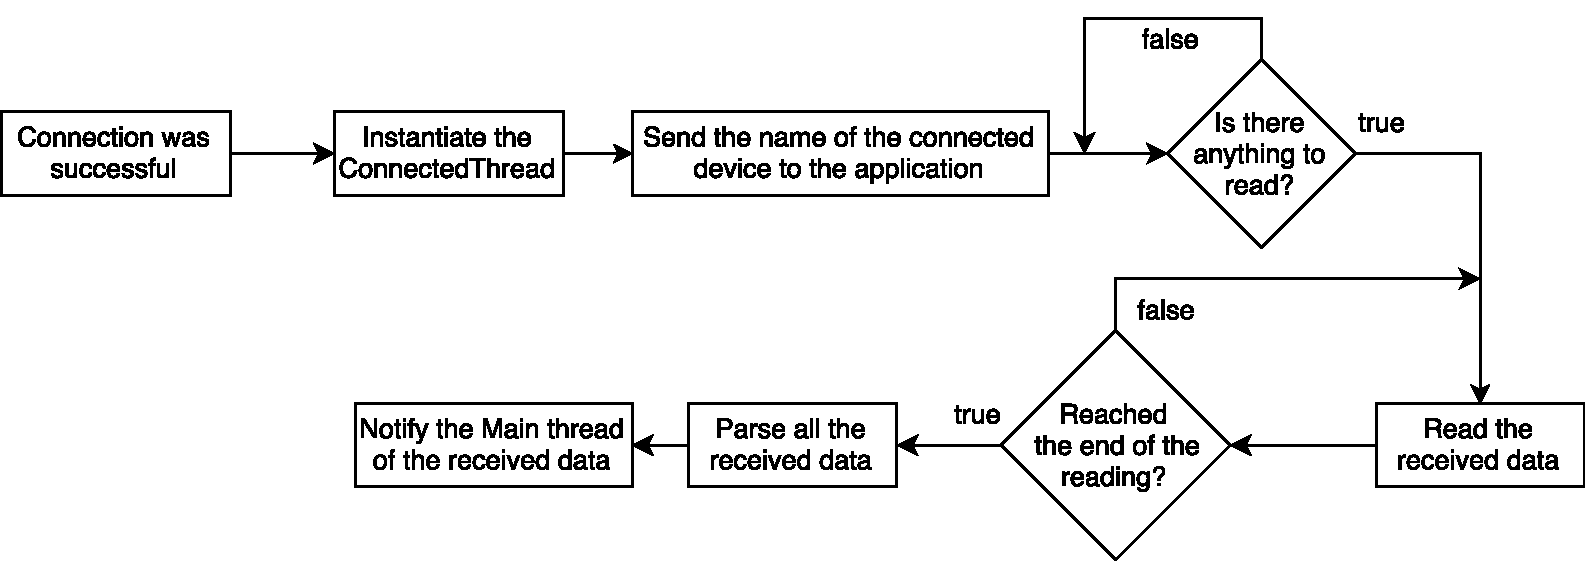
\includegraphics[width=1\textwidth]{images/btconnectedr.pdf}}
	\caption{\label{fig:btconnectedr} Flow diagram of the performed actions of a device reading from a Bluetooth communication socket.}
\end{figure}

\begin{figure}[ht]
	\noindent\makebox[\textwidth]
	{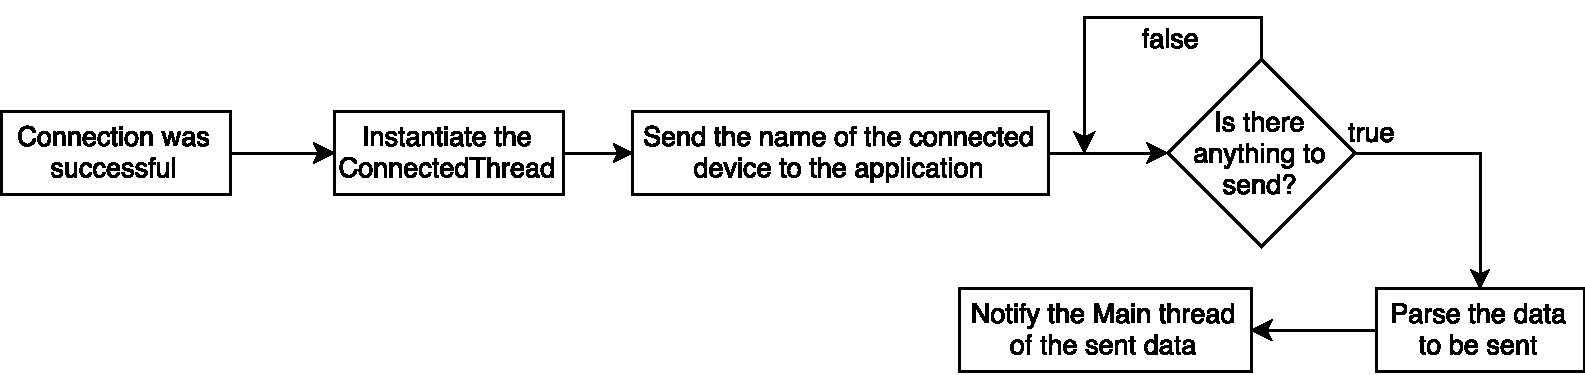
\includegraphics[width=1\textwidth]{images/btconnectedw.pdf}}
	\caption{\label{fig:btconnectedw} Flow diagram of the performed actions of a device writing to a Bluetooth communication socket.}
\end{figure}

To send and receive different data formats within the same application, it is needed to develop a protocol to support the required multiplexing functions. Further along this chapter it will be explained how this was done in the developed application to exchange both text messages and web pages.

\subsection{Discovery and Advertisement Protocol}
\label{subsec:disandadv}

In order to reach an hotspot, a device must first fill its routing table. This process is done by a series of neighbor discoveries\footnote{Discovery is the act of finding nearby devices with Bluetooth on.} and advertisements\footnote{Advertisement is the act of notifying peer devices of the cost of relaying a Request message to the device issuing the advertisement.}, explained in Subsection \ref{subsubsec:disc} and \ref{subsubsec:sendadv}, respectively. Each device will advertise its best estimate to reach the Internet. This advertisement will be processed by peer devices, helping them to fill their own routing tables with the best possible routes.

In Figure \ref{fig:advmsg} the format of an Advertisement message is shown. The type is a feature common to all messages exchanged in this application. It servers the purpose of identifying which type of message is being received. It can take four different values: \textit{ADV}, \textit{RQT}, \textit{RSP} and \textit{FAIL} for an Advertisement, Request, Response and Fail message, respectively. In this case it will take the value \textit{ADV}. The Bluetooth \gls{MAC} identifier is always the \gls{MAC} address of the Bluetooth adapter of the sender. It is then used by the receiver to populate its routing table. Finally, the estimated number of hops is the lower number of hops that separate the sender from the Internet Access Point plus one hop, corresponding to the connection between sender and receiver.

\begin{figure}[ht]
	\noindent\makebox[\textwidth]
	{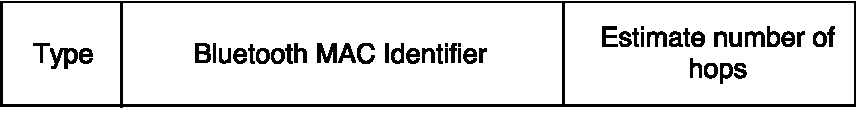
\includegraphics[width=0.7\textwidth]{images/adv_message.pdf}}
	\caption{\label{fig:advmsg} Advertising message format.}
\end{figure}

Each device has two different routing tables: one that is used to store the information retrieved from the advertisement process, providing the best path for routing the Request messages to the Internet Access Point; another used to route a Response message back to the original sender of the Request message that originated the Response, as explained in the next subsection. For simplicity, the first routing table will be referred as Routing Table, while the second will be referred to as Response Table, since it handles the routing of Response messages. 

\begin{table}[ht]
\centering
\bgroup
\def\arraystretch{2.5}
\begin{tabular}{|c|c|}
\hline
\textbf{Next hop node (MAC address)} & \textbf{Number of hops} \\ \hline
Own MAC address & 0 or 16 \\ \hline
Device A's MAC address & Estimate through A \\ \hline
Device B's MAC address & Estimate through B \\ \hline
... & ... \\ \hline
Device Z's MAC address & Estimate through Z \\ \hline
\end{tabular}
\egroup
\caption{Routing Table example and format}
\label{tab:routTables}
\end{table}

In Table \ref{tab:routTables}, an example of a Routing Table is presented, where the first entry is always populated with the device's own \gls{MAC} address and its hop distance estimate, which is either 0 or 16\footnote{16 was chosen to be the representation of infinity or inability to reach a destination, since it has been represented by this number in various protocols, for instance in \gls{RIP}, see \cite{ripprotocol}}, meaning the device has an Internet connection or not, respectively. Every time a device receives an Advertisement message, it populates this table, either by adding a new row or updating an existing one, with the information contained in the message - see Figure \ref{fig:advmsg}. When the routing table is done being populated, each node knows its immediate peers and the best estimate through each one of those peers, giving it a full knowledge of its vicinity, \textit{i.e.}, the sub-network created by the peers that are reached by the device using a single hop.

It is important to start by understanding how the routing tables are created and, then, how and when they are populated. Both tables follow the same principle: they are objects that relate keys to values. To a single key corresponds a single value, thus not creating duplicate entries.

In the scope of this subsection only the Routing Table will be explained - see Subsection \ref{subsec:exch} for the description of the Response Table. The keys of this table correspond to the \gls{MAC} address of the next hop while the values correspond to the respective estimated number of hops. When querying the table for a specific \gls{MAC} address it should return one and only one estimate for the number of hops.

There are three important things that the application needs from this table (1) to get the absolute minimum hop distance estimate to the Internet Access Point, in order to retrieve the device's best path; (2) to get the corresponding key to the minimum hop distance estimate to the Internet Access Point, in order to retrieve the receiver to whom this device should send the message; (3) to update or add a row with a new key-value pair, in order to add newly received advertisement information.

To be able to get the absolute minimum of the estimated number of hops, it is necessary to compare all the existing values of the table. Since it only contains the information of its immediate peers, this process is fast and does not interfere with the rest of the application.

Having the minimum hop distance estimate to the Internet Access Point from the Routing Table, the \gls{MAC} address associated with that entry is retrieved. This \gls{MAC} address belongs to the device providing the best next hop to reach the Internet Access Point.

Finally, the addition and update of Routing Table rows is done whenever an Advertisement message is received. The advertisement provides the \gls{MAC} address and estimated number of hops. Having this information, it is possible to insert the retrieved key-value pair into the existing table. As mentioned before, one key maps to a single value, thus in case this key already maps to a value, the latter will be overwritten with the new one. In case the key does not exist, a new row is created mapping the key to its specific estimated number of hops. Note that, in case of a table update, the application does not compare values, \textit{i.e.}, it does not check if the new estimated number of hops is better than the previous one, since the previous route may have been broken and thus the sender of the Advertisement message always advertises the most recent one.

Since the maximum number of hops to reach an Internet Access Point is capped at 16, the problem of a request being in an infinite loop does not apply. However, if a route link is broken, \textit{i.e.}, a device in the routing path is disconnected or moves out of range, the request will fail until a better estimated number of hops is advertised - see Subsection \ref{subsubsec:sendrqt}, for the failing notification process. To avoid the permanent failure of a request sending, the discovery and advertisement process is repeated in a certain amount of period (default time period is 5 minutes), refreshing the Routing Table.

\subsubsection{Discovering Peers}
\label{subsubsec:disc}

Now that the Routing Table access and modification mechanism is explained, it is possible to discuss where and when it is useful. However, before that, there are still some indispensable features that need mentioning:

\begin{itemize}
	\item During the peer discovery process, several peers may be found, making it necessary to create a place to store them, for further examination. To achieve this a list of neighbor Bluetooth devices is created, where each device corresponds to a found peer in the discovery process. This list is then used to retrieve information from these devices, in order to successfully establish communication sockets with them.
	
	\item To prevent the discovery process of dragging for longer than expected, using processing resources and damaging the performance of the rest of the application, it is necessary to identify if this process is finished and notify the \textit{Main} thread.
\end{itemize}

Figure \ref{fig:discflux} depicts the sequence of actions that the application executes to successfully perform the discovery process.

\begin{figure}[ht]
	\noindent\makebox[\textwidth]
	{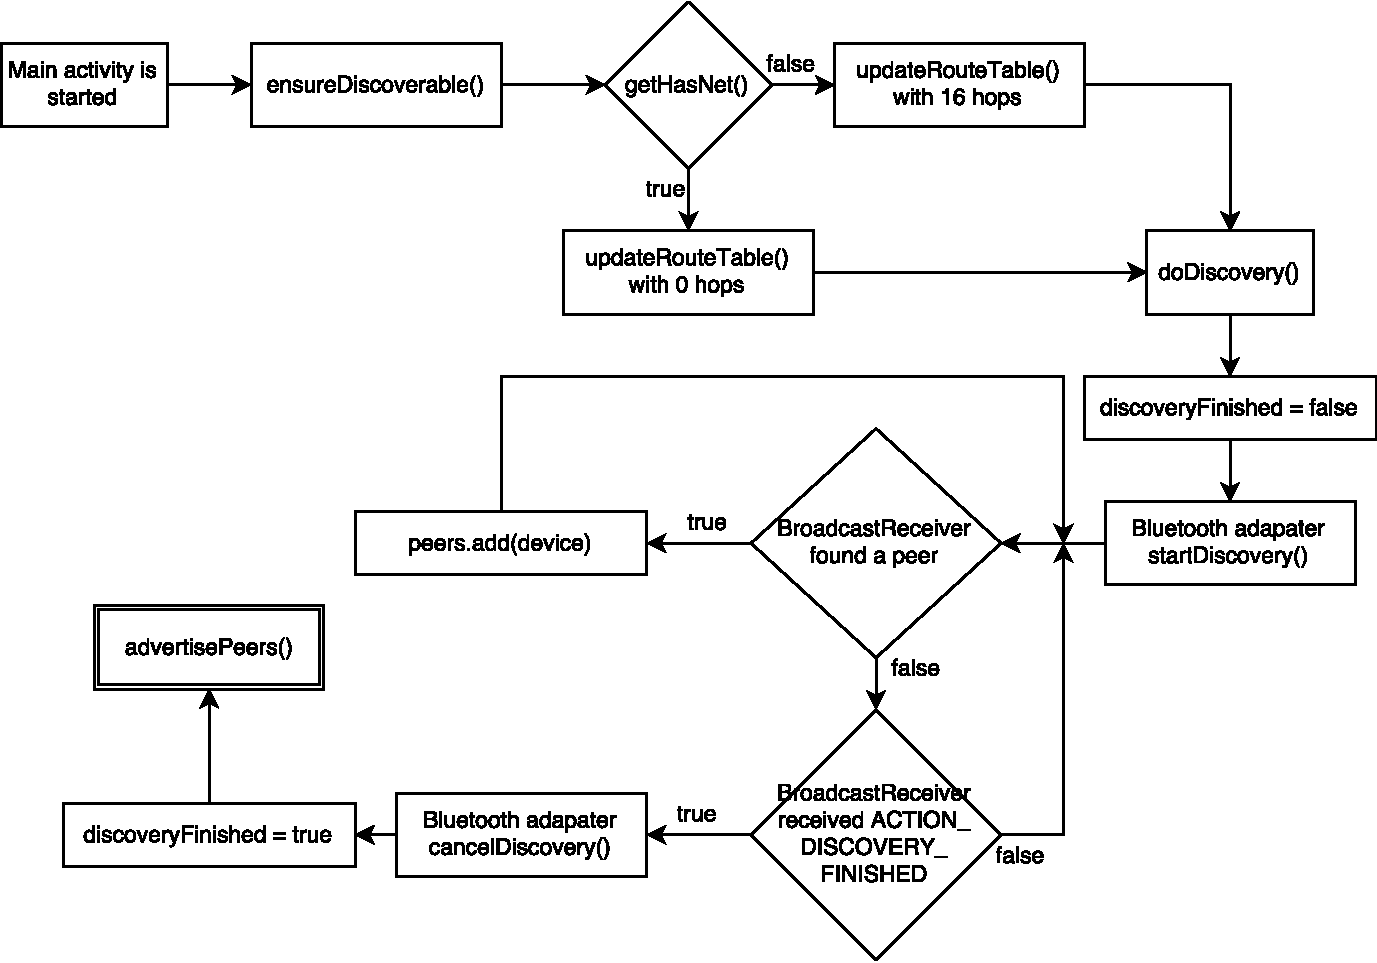
\includegraphics[width=1\textwidth]{images/discovery_flux.pdf}}
	\caption{\label{fig:discflux} Flow diagram of the discovery process.}
\end{figure}

Before beginning the discovery process, the application needs to ensure that all the conditions are met. The Bluetooth status is the first to be checked. The device should have Bluetooth enabled and it should be discoverable for an unlimited amount of time. If the Bluetooth is not enabled, the device cannot begin the discovery process and if the device is not discoverable its peers are not able to send their advertisement to it.

Once the Bluetooth is set up, the initial update of the Routing Table is performed. A quick network check indicates if the device has an active Internet connection. If this is the case, it will add a new row to the routing with its own \gls{MAC} address and 0 hops. Otherwise, it means that the device is currently unable to establish an Internet connection. The same process is performed but, instead of 0 hops, the hop distance estimate will be of 16 hops, for reasons already explained.

The device is now finished with the first step of advertisement, filling the Routing Table with its own \gls{MAC} address and estimate. It is now possible to start the discovery process and advertising this same hop distance estimate to the discovered peers.

Figure \ref{fig:adveg1} demonstrates two devices, one without an Internet connection (left) and one with an active Internet connection (right). At this point both devices should have exactly one entry at their Routing Tables, since they have not communicated with any other device, but they have established their position in the network, \textit{i.e.}, whether they have an Internet connection. Device A is unable to reach the Internet, so it adds to the Routing Table an entry with its own \gls{MAC} address and a number of hops estimate of 16. Device B, on the other hand, is able to directly reach the Internet, thus having an entry with its own \gls{MAC} address and a number of hops estimate of 0.

\begin{figure}[ht]
	\noindent\makebox[\textwidth]
	{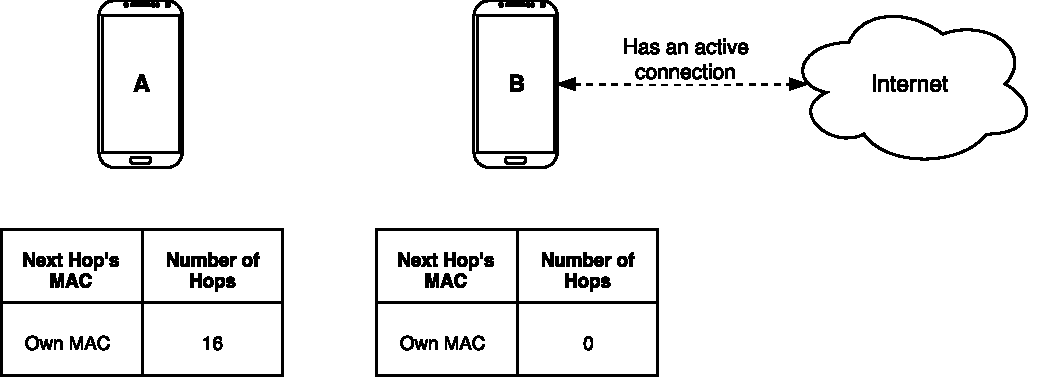
\includegraphics[width=1\textwidth]{images/adv_example_1.pdf}}
	\caption{\label{fig:adveg1} Example 1: State of the two devices after the initial step of the advertisement process is over.}
\end{figure}

The management of the discovery process is relatively simple: the receiver needs to be able to assess the discovery process status, \textit{i.e.}, if it is starting, running or finished. The management of peer discovery is more complex: the receiver needs to retrieve each peer's information and store it in the peer list previously mentioned. A new entry is added only if an entry for the same peer is not already included in the table. Once the discovery is finished, the receiver needs to be able to notify the rest of the application that it can proceed with the advertisement process.

\subsubsection{Sending an Advertisement Message}
\label{subsubsec:sendadv}

The discovered peers are now stored and the device can start the advertisement process. The peer list is iterated through and each item is analysed to understand if it should receive an Advertisement message or not. The analysis consists of checking if the peer fits in the desired category: in this case a smart phone using the developed application.

In Figure \ref{fig:advflux} the flow diagram of the advertisement process is presented.

\begin{figure}[ht]
	\noindent\makebox[\textwidth]
	{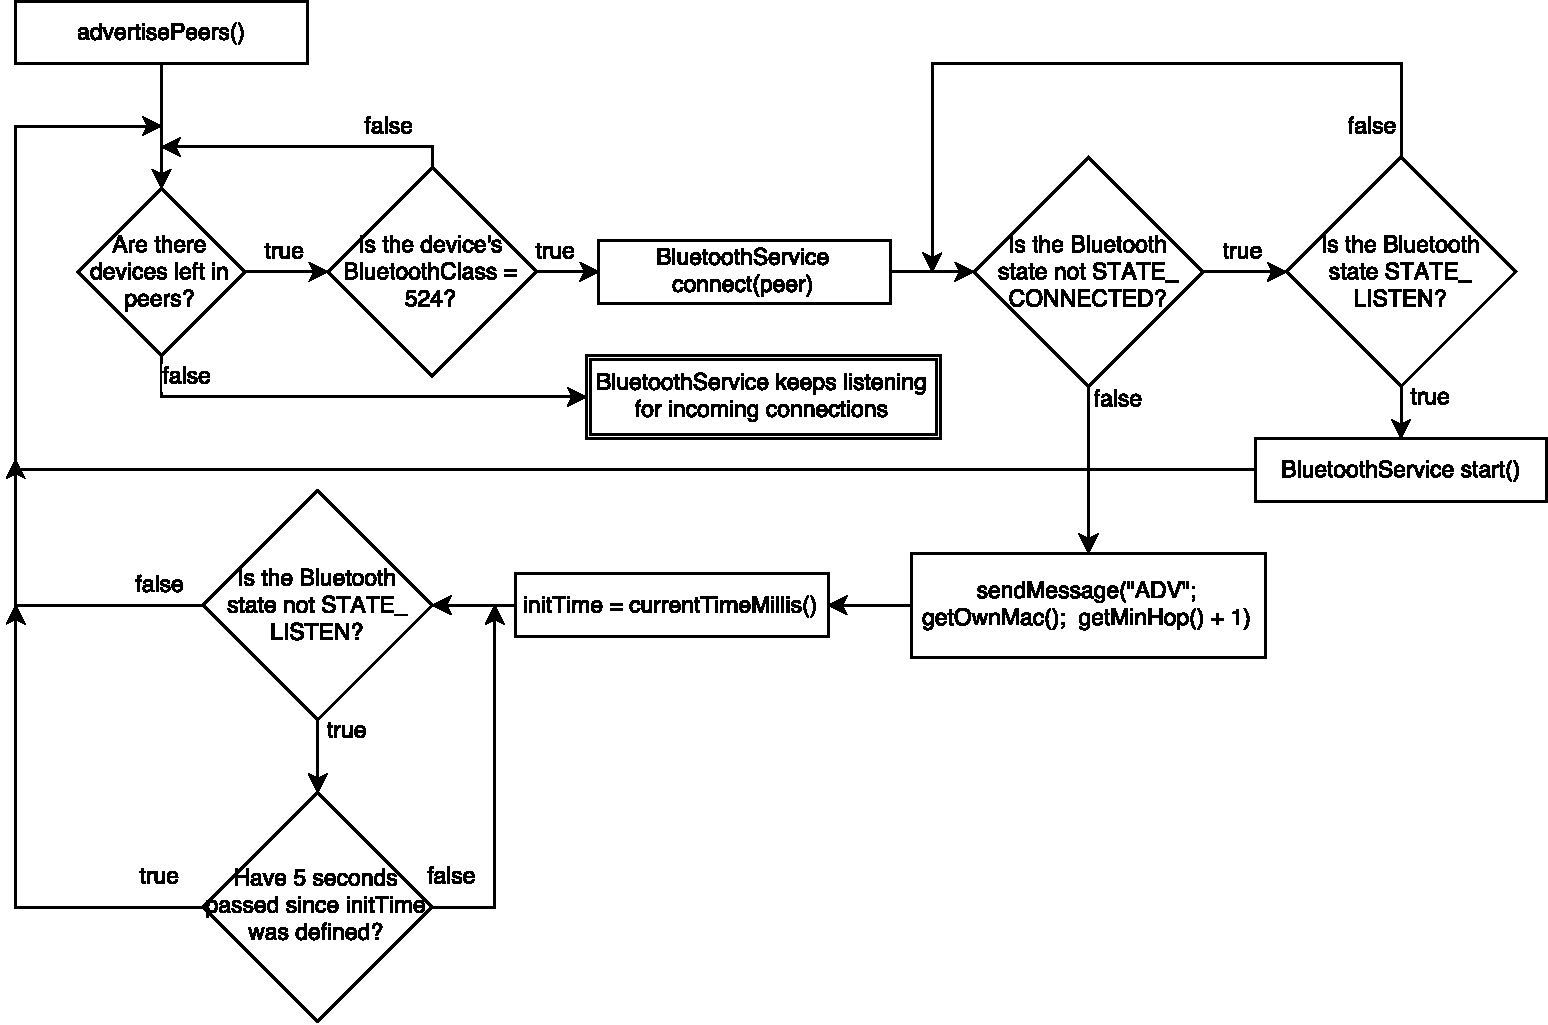
\includegraphics[width=1\textwidth]{images/advertise_flux.pdf}}
	\caption{\label{fig:advflux} Flow diagram of the advertisement process from the point of a sender.}
\end{figure}

Since the number of Bluetooth devices is growing, it is plausible that the discovery process found a peer that does not fit into the desired category, such as a sensor or an headset. To avoid this, a verification is performed to assess if the peer is a smart phone. Overlooking this may be costly in terms of time and computing as the number of attempted connections will increase.

Once the necessary checks are performed and the peer device is eligible to receive an Advertisement message, the device attempts to establish a Bluetooth connection, using the mechanism described in \ref{subsec:btconn}. Before sending the Advertisement message, the application needs to ensure the connection has been successfully established and both devices are ready to write and receive bytes, through the respective streams.

If the conditions to send the message are met, the device queries its Routing Table for the minimum estimated number of hops, explained in Subsection \ref{subsec:disandadv}. This value is incremented and added to the avertisement message. The Advertisement message is then sent, following the format seen in Figure \ref{fig:advmsg}, where the Bluetooth \gls{MAC} identifier is the device's own \gls{MAC} address. This process is then repeated for each peer device found.

\subsubsection{Receiving an Advertisement Message}
\label{subsubsec:rcvadv}

In Figure \ref{fig:recvadvflux} a simplified flow diagram of the actions taken by the receiver of an Advertisement message is shown.

\begin{figure}[ht]
	\noindent\makebox[\textwidth]
	{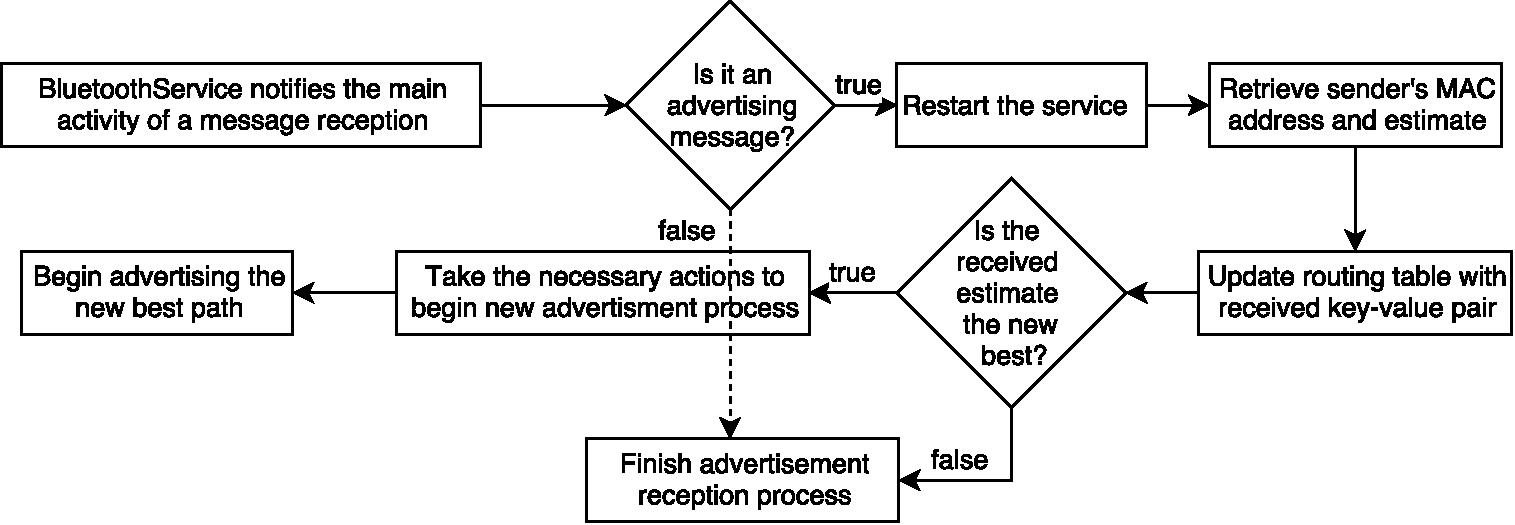
\includegraphics[width=1\textwidth]{images/recv_advertise_flux.pdf}}
	\caption{\label{fig:recvadvflux} Flow diagram of the advertisement process from the point of a receiver.}
\end{figure}

On the advertisement receiver device, the \textit{BluetoothService} notifies the main activity of the message reception and, as mentioned before, this is achieved via a handler, used to pass the received message from the \textit{BluetoothService} to the main activity.

Once the main activity is notified of the message reception, it analyses the context of the application, \textit{i.e.}, which data format is the application expecting to receive at that specific point in time. Since this subsection's scope is the advertisement process, only text messages are expected to be sent and received.

The connection to the advertiser is no longer required, thus the \textit{BluetoothService} is restarted in order to allow the device to start listening to incoming connections. Simultaneously, the received text message is submitted to analysis, in order to identify what type of message has the device received, from the different possibilities: Advertisement, Request, Response or Fail message.

By analysing the type field present in the message, see Figure \ref{fig:advmsg}, the message is identified as an Advertisement message and submitted to the chain of actions specific to that message type. The first step is to extract the information contained in the message, \textit{i.e.}, the sender's \gls{MAC} address and the estimated number of hops to reach the Internet.

Having these values, the device compares the received hop distance estimate with the best from the ones stored in the Routing Table, process described in Subsection \ref{subsec:disandadv}. If the comparison concludes that the received hop distance estimate is not smaller than the current best, a new entry is added to the Routing Table is added with the received hop distance estimate and \gls{MAC} address, since it provides a possible alternative route if the current best path to reach the Internet Access Point is broken.

Otherwise, if the received hop distance estimate provides a better path to reach the Internet Access Point, the Routing Table is updated, the device then takes the necessary steps to start a new advertisement process, this time advertising the new best hop distance estimate, previously described. 

In Figure \ref{fig:adveg2}, the example from Subsection \ref{subsubsec:disc} is extended.

\begin{figure}[ht]
   \noindent\makebox[\textwidth]
    {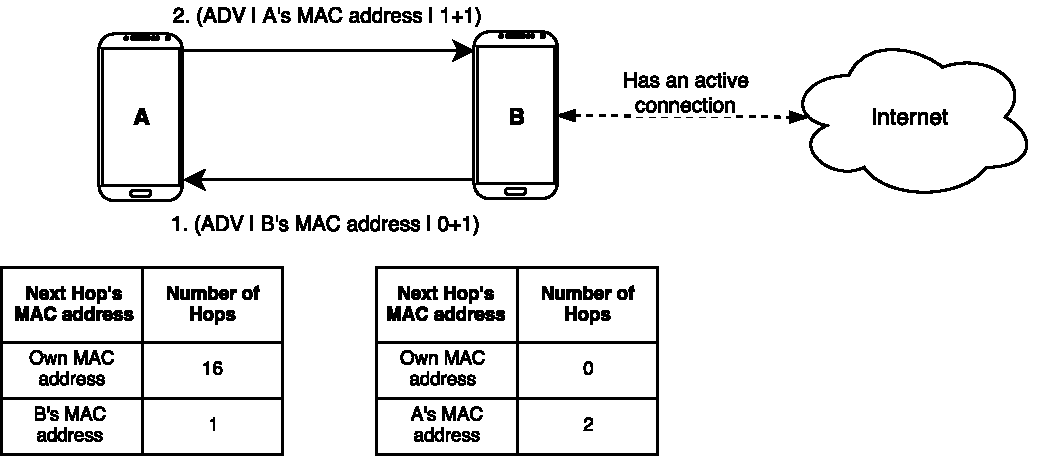
\includegraphics[width=1\textwidth]{images/adv_example_2.pdf}}
	\caption{\label{fig:adveg2} Example 1: State of the two devices after the advertisement process is concluded.} 
\end{figure}

Now, device B has advertised to its peers, which include device A. Upon receiving this message, device A proceeds to store the information in its Routing Table, followed by an advertisement from itself, since the new hop distance estimate is better than the previous one. After this process is concluded, both devices have the Routing Tables displayed in Figure \ref{fig:adveg2}.

If A advertises first, the result will be the same, since when B is advertising, A will still receive a better hop distance estimate and advertise again. When B receives the second Advertisement message from A it will overwrite the previous entry, maintaining the same values.

After the discovery and advertisement phases, each device has a full view of its vicinity and it is possible to establish a network for Internet access using the best possible path. The next subsection will refer to the next step, where the devices already have their Routing Tables populated and are ready to exchange web pages.

\subsection{Web Page Exchange Protocol}
\label{subsec:exch}

This subsection will cover the developed web page exchange protocol. To manage the exchange of the web pages, two messages are exchanged between devices (1) a Request, containing the web page's \gls{URL}, which is sent from the request initiator to the Internet Access Point; (2) a Response message, managing the return of the web page, guaranteeing it follows the correct path to its destination. The Response message will follow the Request's inverse path, starting in the Internet Access Point and ending in the request initiator.

To aid devices sending Response messages in the correct path, a Response Table is created. Once a device has received a Request message and it has an Internet connection, it simply sends back the Response message from where it received the Request. But, in the case this device is a "bridge" node, \textit{i.e.}, a node that forwarded a Request message, with no direct Internet connection, it may have received requests from different devices and it still needs to be able to differentiate each message and decide which device to send back the Response message to.

The Response Table has a similar structure to the Routing Table but it serves a different purpose. In Table \ref{tab:rspTables} it is possible to see the structure of the Response Table.

\begin{table}[ht]
\centering
\bgroup
\def\arraystretch{2.5}
\begin{tabular}{|c|c|}
\hline
\textbf{Message ID} & \textbf{Next hop node (MAC address)} \\ \hline
Message ID \#1 & Device X's MAC address \\ \hline
Message ID \#2 & Device Y's MAC address \\ \hline
Message ID \#3 & Device Z's MAC address \\ \hline
... & ... \\ \hline
Message ID \#9 & Device X's MAC address \\ \hline
\end{tabular}
\egroup
\caption{Response table example and format}
\label{tab:rspTables}
\end{table}

Despite having similar structures, the two tables store different information: the Routing Table maps a \gls{MAC} address to an hop distance estimate, whereas the Response Table maps a message identifier to a \gls{MAC} address. Hence, the need of having two distinct tables.

Two main actions are allowed in a Response Table:

\begin{itemize}
	\item To add new rows and to retrieve the next hop's \gls{MAC} address for a certain message identifier. The message identifiers are random numbers ranging from -2\textsuperscript{31} to 2\textsuperscript{31}, providing around 4.3 billion possible numbers. Since the message identifiers are unique, the existing Response Table rows are never modified, only new ones are added.
	
	\item Given a message identifier, the next hop's \gls{MAC} address should be returned. Since to a message identifier corresponds a single \gls{MAC} address there should be no problems in the response path. However, in case the requested message identifier is not found in the Response Table, the application is notified that the response can not be routed due to the lack of a next hop \gls{MAC} address.
\end{itemize}

Figure \ref{fig:example1.0} presents an example with three devices: A, B and C. Device C has an active Internet connection. The figure also shows the routing tables of each device after the discovery and advertisement processes are completed. Device A will choose B to send a Request message and B will choose C, since they provide the best estimates, respectively.

\begin{figure}[ht]
	\noindent\makebox[\textwidth]
	{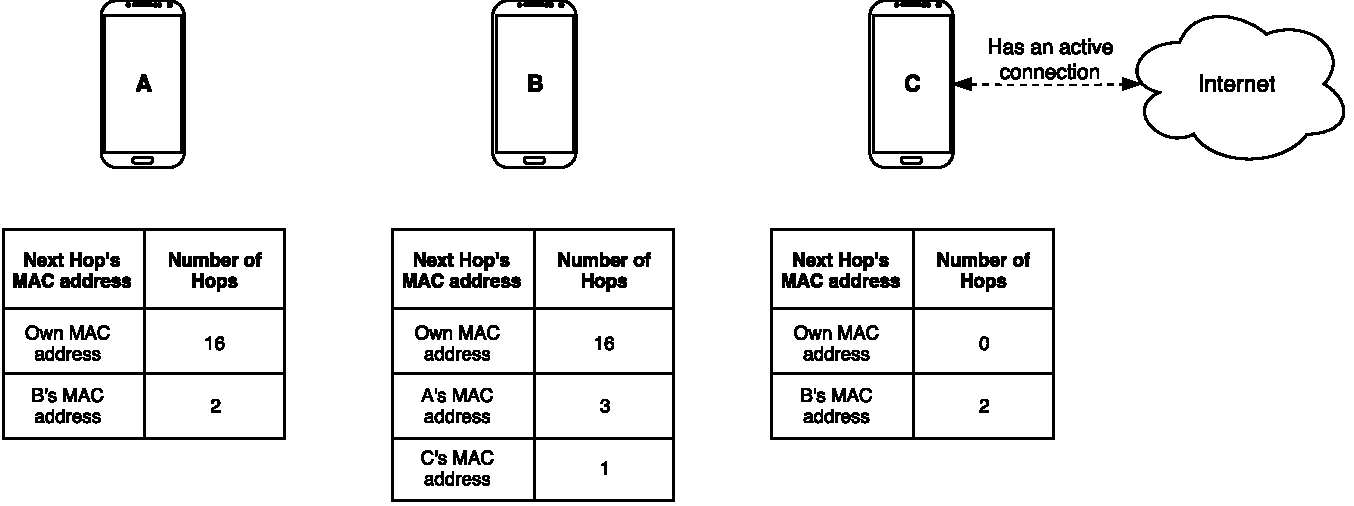
\includegraphics[width=1\textwidth]{images/example_1_0.pdf}}
	\caption{\label{fig:example1.0} Example 2: State of the routing tables of the three devices.}
\end{figure}

\subsubsection{Sending a Request Message}
\label{subsubsec:sendrqt}

The exchange of web pages requires a number of features that need to be mentioned before further explanation:

\begin{itemize}
	\item  A text area enabling the input of a \gls{URL} from the application user.
	
	\item A button for the user to notify the application that he/she has finished inputting the desired \gls{URL}. This button will act as a trigger for the application to begin the request sending.
	
	\item A mechanism to manage the actions related to web pages must be created. In this thesis the method found that best fit the requirements was the creation of a \textit{WebView} instance.
	
	\item A handler providing the link between the \textit{BluetoothService} and the main activity, previously mentioned in the context of the advertisement process, that can communicate the bytes received by the service to the rest of the application.
	
	\item Finally, a mechanism to identify how the received bytes should be processed, \textit{i.e.}, what format should they be converted into. This mechanism must also provide a method to parse the protocol messages and instruct the application to act accordingly, \textit{i.e.}, to follow a specific set of actions depending on the message type.
\end{itemize}

In Figure \ref{fig:rqtflux} a flow diagram representing the request sending process is shown. It provides a visual overview of the application workflow when user input triggers the request sending mechanism.

\begin{figure}[ht]
	\noindent\makebox[\textwidth]
	{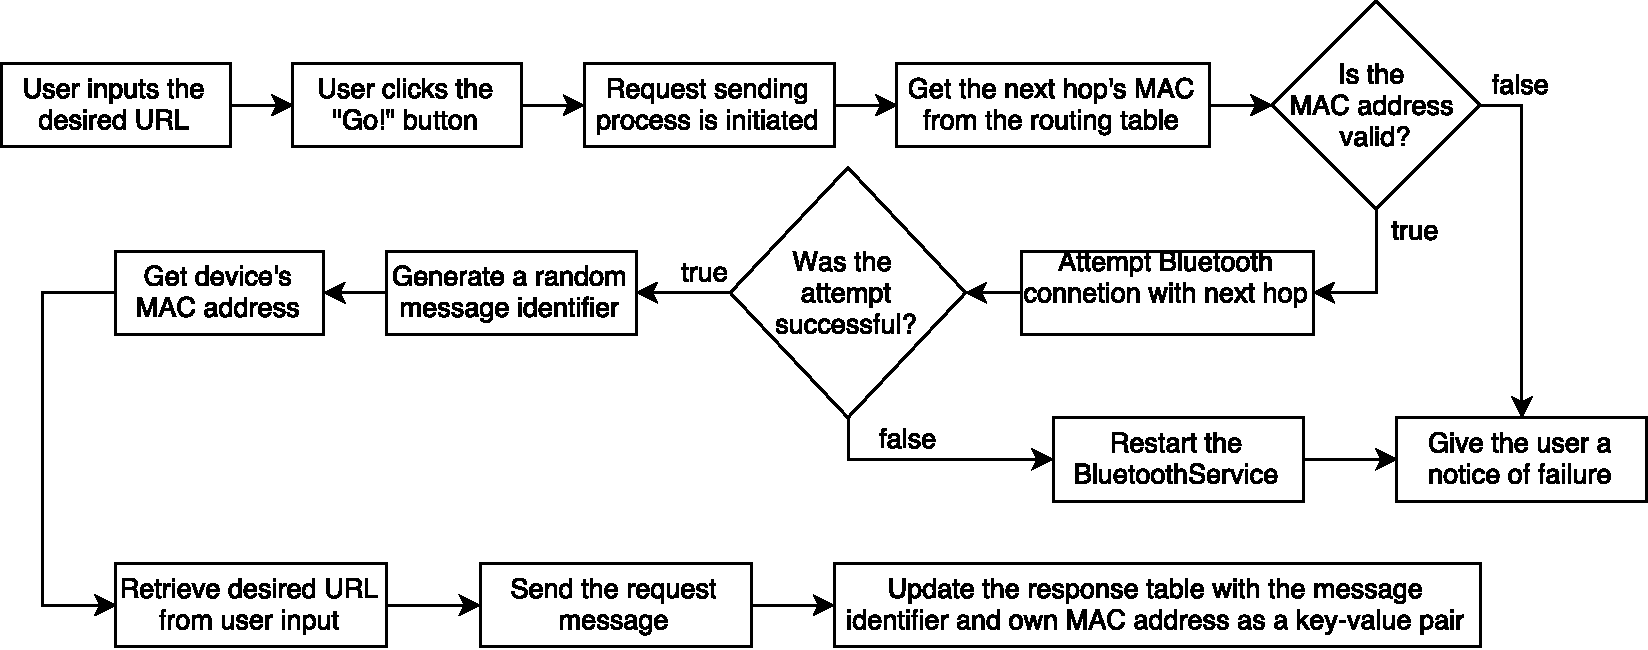
\includegraphics[width=1\textwidth]{images/rqtflux.pdf}}
	\caption{\label{fig:rqtflux} Flow diagram of the request sending process triggered by user input.}
\end{figure}

Assuming the device already established the best route to reach the Internet, \textit{i.e.}, its routing table is populated, the journey of the web page request from the user input to the display of the response will be explained.

In Figure \ref{fig:rqtmsg}, a generic Request message is shown. Its format does not differ much from the one presented in Figure \ref{fig:advmsg}. However, two new fields are introduced: the \textit{Message ID}, a unique identifier representing each message that will be useful to keep track of what is each message's payload and sender, and the \textit{\gls{URL} to request}, which is the \gls{URL} the user is trying to access.

\begin{figure}[ht]
	\noindent\makebox[\textwidth]
	{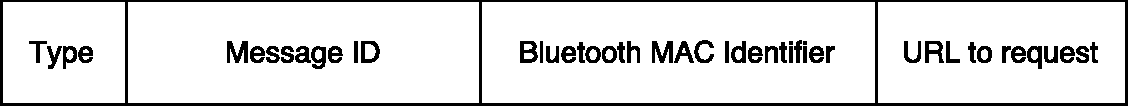
\includegraphics[width=0.9\textwidth]{images/rqtmessage.pdf}}
	\caption{\label{fig:rqtmsg} Request message format.}
\end{figure}

The web page request process may be initiated by two different events: when the user inputs an \gls{URL} and presses the "Go!" button, or when the device receives a Request message and its next action is to forward it to the next hop.

Assuming the originating event is correctly identified and the process is aware that it was initiated by user interaction, the first action is to retrieve the next hop's \gls{MAC} address, to whom the device shall send its request. This can be achieved by using the routing table retrieving the best next hop candidate to reach the Internet.

If the routing table query does not return a valid \gls{MAC} address, the user is notified of the request failure. If a valid \gls{MAC} address for the next hop is returned, the device attempts to establish a connection with the next hop, following the same mechanism as in the advertisement process. Should the connection attempt fail, the user is notified of the request failure, allowing him/her to restart the request process. In that case, the \textit{BluetoothService} is also restarted to keep the device listening to incoming connections.

If the connection is successfully established, the application will proceed to the generation of the Request message to be sent.

Once the Request message is sent, the application updates its Response Table with the generated message identifier and the \gls{MAC} address of the sending device, \textit{i.e.}, its own \gls{MAC} address, as a key-value pair. With this mechanism the device is able to assess if it is the destination of a certain response or if it is a relay node that should forward the response to the next hop. This assessment will be presented and explained in \ref{subsubsec:rcvrqt}.

If the request sending device is forwarding a received Request message, there is no random identifier generation, since the value will be retrieved from the received Request message. Also, the Response Table is not updated because this will be done during the reception process, explained in the next subsection.

However, if the connection establishment fails, the user is not notified, since this Request message was not originated by him/her. In this case, the device queries the Response Table for the \gls{MAC} address mapped by the Request message identifier, corresponding to the device that sent/forwarded the Request message to this node. A failure notice is then sent to that device, with the intent of notifying the Request message originator about the inability to forward the request until it reaches the Internet.

If the connection is successfully established, the message is sent as before, with the slight difference that the message identifier and the \gls{URL} to be requested are retrieved from the values encapsulated in the received Request message - see Figure \ref{fig:rqtmsg}.

\subsubsection{Receiving a Request Message}
\label{subsubsec:rcvrqt}

The request reception process similar to the advertise receiving. The device receives a connection attempt from a peer. If the connection is successfully established, the Request message is received by the device in \textit{BluetoothService}.

In Figure \ref{fig:rqtrcvflux} it is possible to see a flow diagram of the request receiving process.

\begin{figure}[ht]
	\noindent\makebox[\textwidth]
	{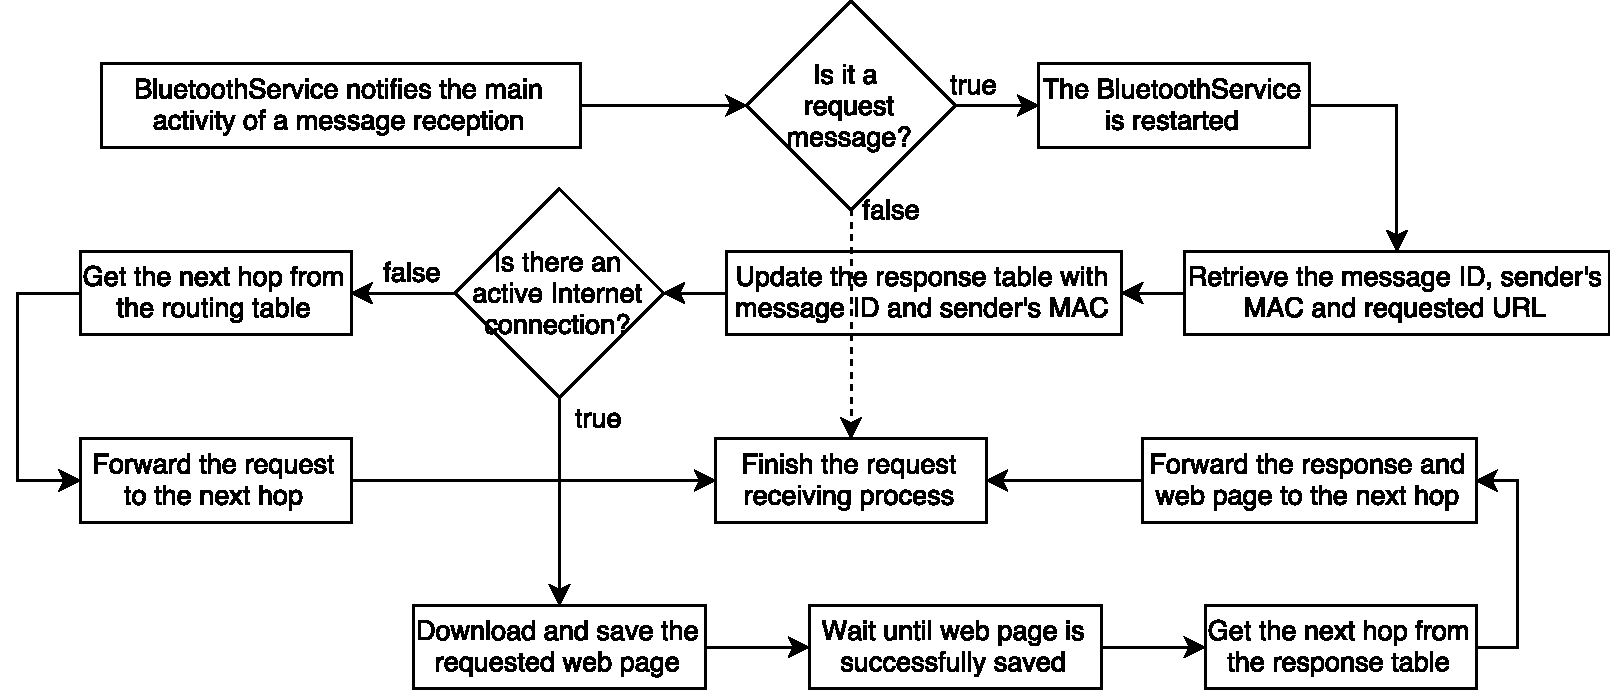
\includegraphics[width=1\textwidth]{images/rqt_rcv_flux.pdf}}
	\caption{\label{fig:rqtrcvflux} Flow diagram of the request receiving process.}
\end{figure}

As in the advertisement reception process, see Figure \ref{fig:recvadvflux}, the received message is classified according the possible types: an Advertisement, a Request, a Response or a Failure. The \textit{BluetoothService} is also restarted.

Once the message is correctly classified, as an Advertisement, the message identifier and sender's \gls{MAC} address are retrieved from the message - see Figure \ref{fig:advmsg}. In the request sending process it was mentioned that in case the device was not the owner of the Request message, it would not update the Response Table. For devices that receive a Request message but are not its originators, the table updating process is done during this phase. Thus, the routing table is updated with the retrieved message fields.

At this point, there are two options of execution: one regarding the devices with Internet connection and another for the devices without one. To define which approach is taken by the device, a quick check of the Internet connection status is performed. If the check returns false, meaning the device has no active Internet connection, the request will be forwarded to the next hop, retrieved from the routing table, towards a device with an Internet connection. To do this, the application proceeds as described in \ref{subsubsec:sendrqt} for a device that is not the owner of the request, where the sent \gls{URL} and message identifier are the ones that were previously retrieved from the received message and the \gls{MAC} address is the device's own address.

On the other hand, if the Internet check returns positive, it means the device is a final destination for the received request. The device will act as a communication link between the Internet and the owner of the request. It now has to retrieve the requested web page and send it backwards until it reaches its original requester.

The methodology to save the web page had several possibilities, such as saving the web page as an image, saving only the \textit{HTML} content or saving each element of the page individually. The first two methods are not complete, meaning the web page could lose some of its features, \textit{e.g.} dynamic images, search fields, \textit{etc.}. The third method would fully download the web page, however it would require additional logic to save the different elements in the same directory and to arrange them to re-create the web page with its initial format. The implemented solution saves the web page as a web archive, which is specific to the \textit{WebView} class - see \cite{webview}. It solves the problem of saving the web page's different elements and re-arranging them to restore the web page, since it downloads each element but compiles them in a web archive, that can be easily decompressed by \textit{WebView}. Thus, it proved to be the best solution.

The thread \textit{WaitForWebPage} (see Figure \ref{fig:appsandbox}), is used to ensure that the web page is successfully saved in the application's file directory. It is specially useful for the download and saving of large web pages where this process can be time consuming. If this thread is not run, the device risks sending a Response message before having the complete web page file, failing to transmit the requested web page to its destination. This process is done concurrently, allowing the application to continue its normal functions, such as listening to incoming connections.

Once the download and saving process is completed, the device must notify the next hop about the file transfer that will occur. For this effect, a Response message is sent to the \gls{MAC} address mapped by the received message identifier from the Request message. If a valid \gls{MAC} address is returned, the device attempts to establish a connection and send a Response message, as explained in the next subsection.

Resuming the example in Figure \ref{fig:example1.0} and supposing the user from device A wants to request a \gls{URL} and inputs it correctly, the device will follow the steps explained in Subsection \ref{subsubsec:sendrqt} and check the routing table to establish the next hop. Also its Response Table will be filled during this action, since it is the owner of the request.

Once that process is completed and the message reaches device B, it will update its routing table with the newly received Request message. After that, it checks its own routing table and assesses if it should forward the request or download the page. Since the device does not have an active connection, the request will be forwarded to C.

Finally, upon receiving the Request message, device C will update its own Response Table with the received message identifier and B's \gls{MAC} address. Since device C has an active Internet connection, it will download the web page.

Figure \ref{fig:example1.1} depicts this process, as well as the three Response Tables from the devices after the Request messages are all sent and the web page downloaded.

\begin{figure}[ht]
	\noindent\makebox[\textwidth]
	{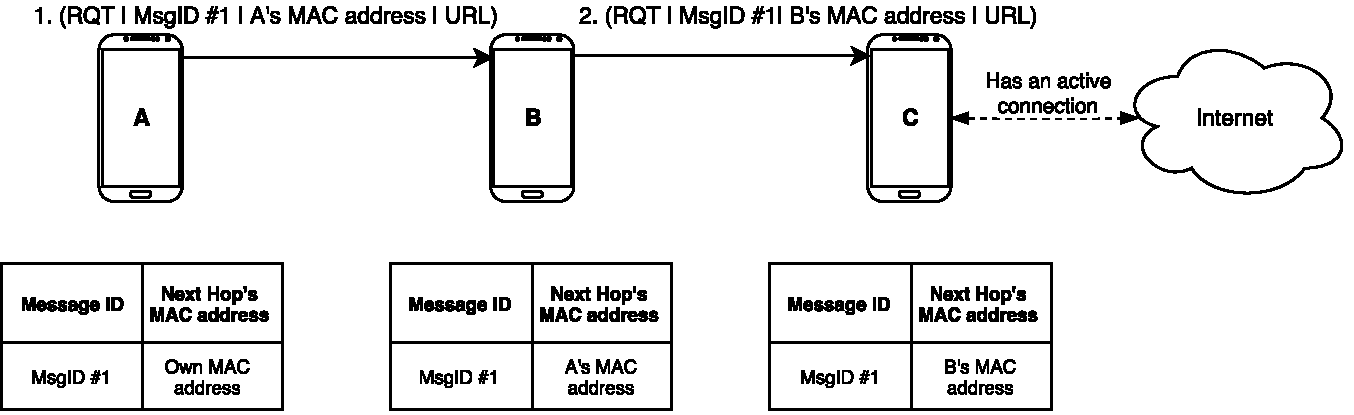
\includegraphics[width=1\textwidth]{images/example_1_1.pdf}}
	\caption{\label{fig:example1.1} Example 2: Request sending and receiving process.}
\end{figure}

\subsubsection{Sending a Response Message and Web Page}
\label{subsubsec:sendrsp}

In this subsection the process of sending a Response message and a web page will be explained. The response will be routed back until it reaches the owner of the request that originated this response. In the previous section the process of receiving a Request message and downloading and saving the web page are explained.

In Figure \ref{fig:rspsendflux} a flow diagram of the Response message and web page sending process is presented. It shows the mechanism from the time the web page is saved, until it is sent. As previously described, the process is finished if no valid next hop for that message identifier is retrieved, or by correctly sending the web page as expected.

\begin{figure}[ht]
	\noindent\makebox[\textwidth]
	{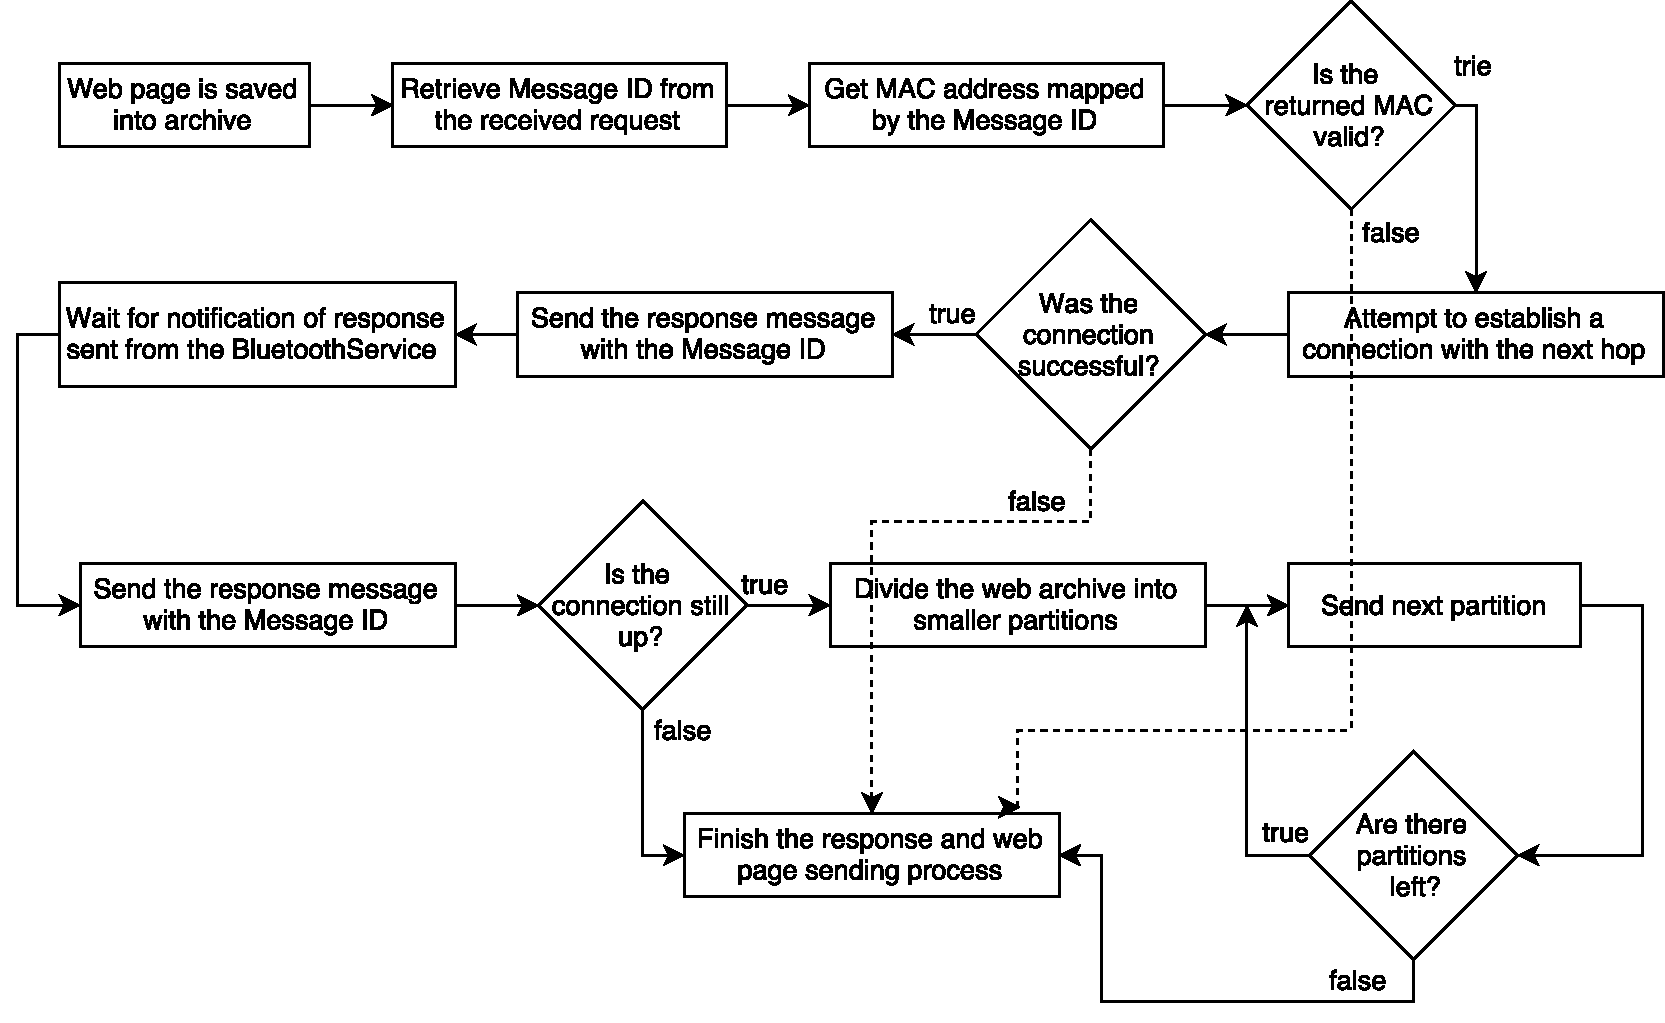
\includegraphics[width=1\textwidth]{images/send_rsp_flux.pdf}}
	\caption{\label{fig:rspsendflux} Flow diagram of the Response message and web page sending process.}
\end{figure}

To send the Response message to the correct destination, the device queries the Response Table for the \gls{MAC} address of the next hop mapped by the message identifier received in the Request message. If a valid \gls{MAC} address is returned, a connection is attempted, as seen in the other sending processes - see Subsections \ref{subsubsec:sendadv} and \ref{subsubsec:sendrqt}.

In Figure \ref{fig:rspmsg} the format of a generic Response message is shown. The \textit{Message ID} will have a direct correspondence with the message identifier of the request that originated this response. The Response message is used as a notification, alerting the receiving device of an incoming web page file.

\begin{figure}[ht]
   \noindent\makebox[\textwidth]
    {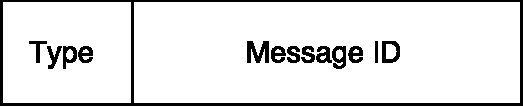
\includegraphics[width=0.4\textwidth]{images/rspmessage.pdf}}
	\caption{\label{fig:rspmsg} Format of a Response message.}
\end{figure}

Once the \textit{Main} thread is notified by the \textit{BluetoothService} that the Response message was correctly sent and received, it must send the requested web page archive to the next hop. This notification is passed from the service to the \textit{Main} thread via the previously mentioned handler.

In this stage, the sending device does not need to attempt a new connection with the receiver - the established connection is maintained open until the web page transfer is complete. To initiate the file transfer, the web archive file must be converted into a byte array, due to the Bluetooth transfer mechanism explained in \ref{subsubsec:connected}. The application then retrieves the archive's file size to match the array size.

The device checks if the established connection is still open. If this is the case, the bytes are then written to the input stream as usual. However, in contrast to what happened with the single text messages, the file bytes can be larger than the connection stream buffer. To overcome this problem, it is necessary to implement the segmentation of large files, \textit{i.e.}, the ones larger than the stream buffer, into smaller partitions. These partitions must be sent individually and, during the reception, they must be regrouped into the original file, as will be shown in the next subsection.

If the connection was shut down due to unexpected behaviour from one of the parts, such as a forced disconnection due to moving out of range, the web archive is not sent, the web page sending process is aborted and the device keeps listening to incoming connections.

\subsubsection{Receiving a Response Message and Web Page}
\label{subsubsec:rcvrsp}

In the receiver side, the web page and Response message are received and the device must assess if it is the final destination or if it is a relay node for a different device, in which case the web page will not be displayed, but the Response message and web page are forwarded.

In Figure \ref{fig:rsprcvflux} a simplified flow diagram of the Response message and web page reception process is shown. It is possible to visualize the file receiving workflow as well as the different possibilities for the receiver of the response: forwarding the response or displaying the web page. It is also shown the mechanism behind the multi-page request. With the shown implementation, the user is capable of seeing the requested web pages and navigate through those pages without having to manually send each request.

\begin{figure}[ht]
	\noindent\makebox[\textwidth]
	{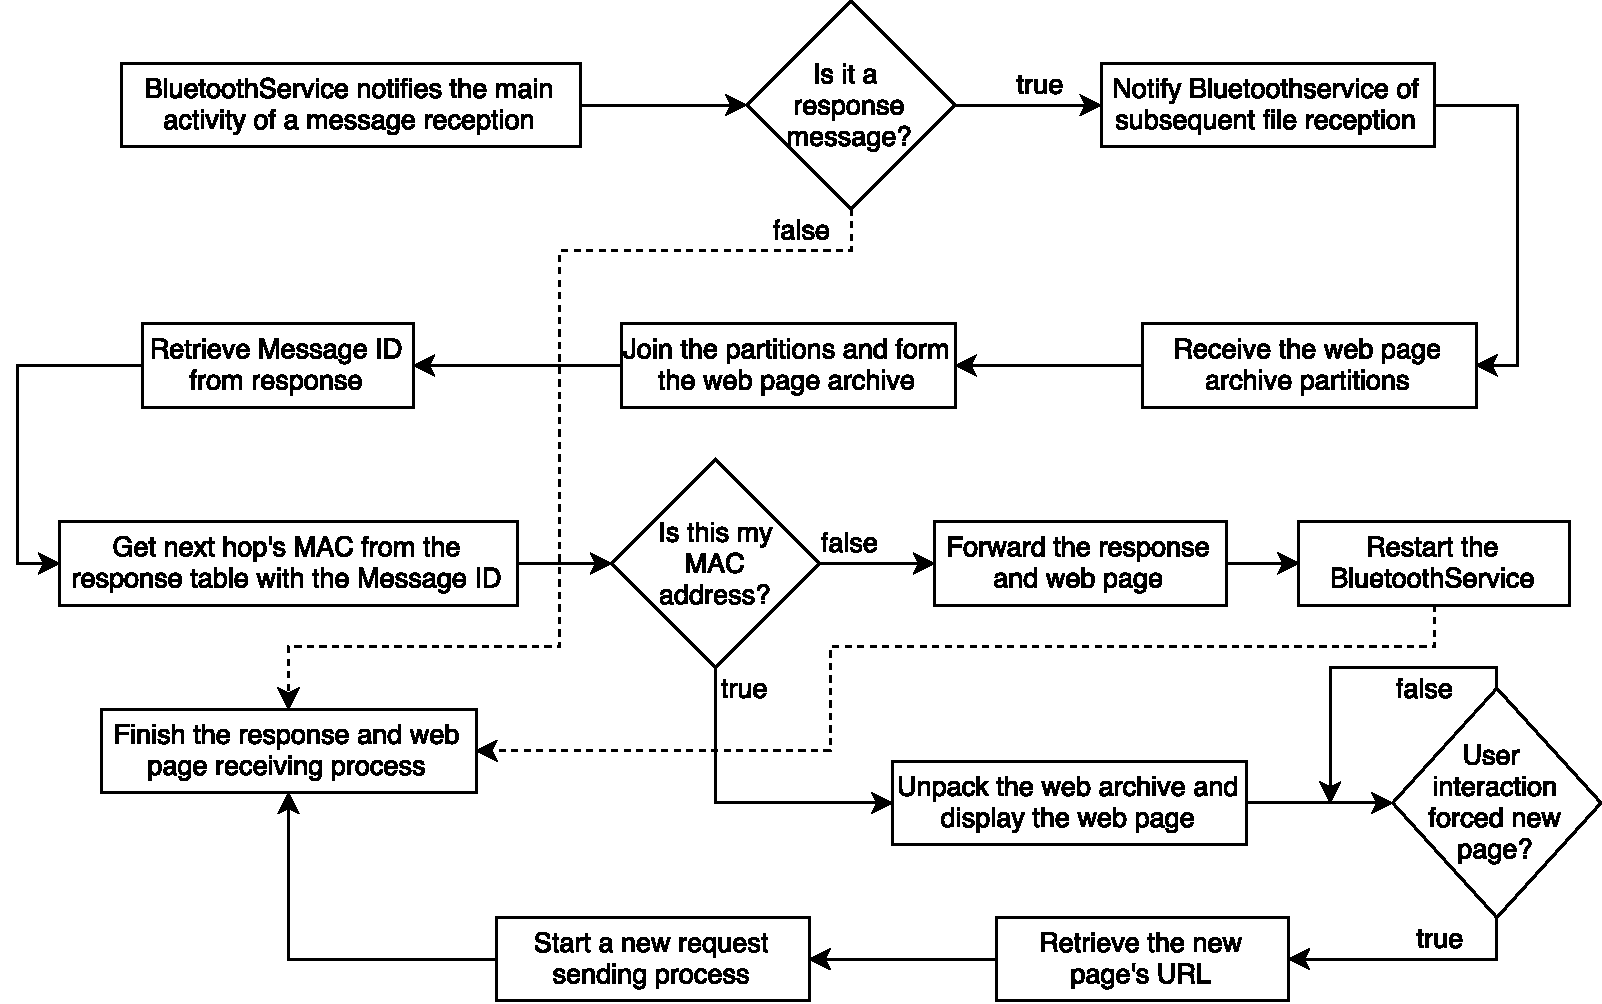
\includegraphics[width=1\textwidth]{images/rcv_rsp_flux.pdf}}
	\caption{\label{fig:rsprcvflux} Flow diagram of the Response message and web page receiving process.}
\end{figure}

This process begins when the handler notifies the \textit{Main} thread that a message has been received. The message is compared with the possible types and is identified as a Response message.

At this point, the device knows it will be receiving a web page archive, so the connection is not shut down as it happens in the advertise and request receiving processes - see Subsections \ref{subsubsec:rcvadv} and \ref{subsubsec:rcvrqt}, respectively. This mechanism allows the application to reduce the duration of the web page exchange.

The \textit{BluetoothService} is notified that the next reception will correspond to a web page archive. Since the connection is still up, new incoming connections will be blocked not allowing other devices to interfere with this exchange until it is completed.

Once the message is identified and passed to the \textit{Main} thread, it will be analysed, \textit{i.e.}, the message identifier will be extracted - see Figure \ref{fig:advmsg}. This is done to retrieve the next hop from the Response Table. Two situations are possible: either the device is the destination of that response or it isn't and the message must be forwarded to the next hop.

The sender will then proceed with the transfer of the web page archive. At this point, the receiver of the web page is aware that a web archive is being transferred, as opposed to a text message. Using the implemented logic in \textit{BluetoothService} for the reception of this data type, the web archive is fully received and transferred to the \textit{Main} thread, through the handler.

Once the \textit{Main} thread is notified about the received web archive, the device saves it in the application's directory. The service is restarted and is now able to receive new connections, changing the receiving logic to the reception of text messages, since it is not expecting to receive more segments for the time being.

The device now has received both the Response message and the web page and it has all the necessary parts to decide which action to take. That is achieved by querying the Response Table with the retrieved message identifier, from the Response message. This query returns a \gls{MAC} address and the application verifies if it is valid or not.

If the \gls{MAC} address is deemed valid a new check is performed, this time with the purpose of assessing if the device is the final destination of the response. If the retrieved \gls{MAC} address does not correspond to its own \gls{MAC} address, meaning this device is not the destination, it attempts to establish a connection with the next hop, identified by the retrieved \gls{MAC} address. If the connection is accepted and established, the Response message and web page sending process is initiated - see \ref{subsubsec:sendrsp}.

On the other hand, if the device is deemed the owner of the request that originated this response, \textit{i.e.}, its \gls{MAC} address corresponds to the one retrieved from the Response Table, it means the web page archive must be unpacked and displayed to the user.

As mentioned before, the \textit{WebView} class is used to manage the actions performed with web page and these ones are no exception. So, the \textit{WebView} is initialized and made visible to the user. The web archive is then unpacked and displayed to the user using methods inherent to this class - see \cite{webview} to learn which ones may be useful for this purpose.

When the user receives the requested web page, he/she might want to navigate through other pages, corresponding to web links in the previous one (for instance when a user clicks in a link present in the web page, requesting a subsequent page). With the current \textit{WebView} implementation, once a web link is clicked, the "no Internet connection" error will be displayed, as it would happen in a normal web browser opened in a device without Internet connection. This lack of continuity severely affects the usability of the application thus, a solution to this problem was developed.

A solution that proved to be effective is to create a mechanism to detect web page loading errors, such as the "no Internet connection" error. Once the mechanism is triggered, meaning an error occurred, the application must retrieve the requested \gls{URL} and form a new Request message from it - see \ref{subsubsec:sendrqt} for the explanation of this process. This mechanism must overwrite the usual action of simply loading the web page, when requested by the user.

With this mechanism, when the requested web page is loaded and displayed to user, he/she is free to interact with the web page as in the case of a normal web browser. Once this interaction leads to a new web page being requested and displayed, the solution's mechanism is triggered and a new Request message is formed and sent, being submitted to the web page exchange process.

To finalize the example from Figures \ref{fig:example1.0} and \ref{fig:example1.1}, device C, after finishing downloading the web page, will check its Response Table and send a Response message to device B, which is the next hop retrieved for that specific message identifier \textit{MsgID \#1}. The Response message is followed by the web page archive, previously downloaded, as described in Subsection \ref{subsubsec:sendrsp}.

Device B receives the Response message and the web page, following the steps previously explained in Subsection \ref{subsubsec:rcvrsp}, and checks its Response Table for that message identifier. Device A's \gls{MAC} is returned from that query and that's the destination for B's response, so device B sends the Response message and web page to A.

Figure \ref{fig:example1.2} illustrates this example and messages exchanged between the three devices, as well as the Response Tables, previously established in Figure \ref{fig:example1.1}.

\begin{figure}[ht]
   \noindent\makebox[\textwidth]
    {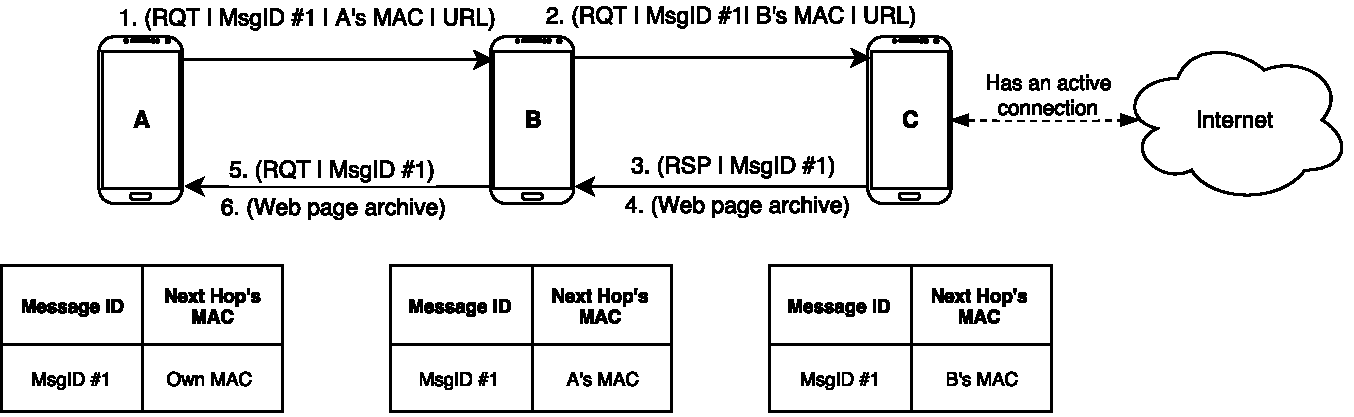
\includegraphics[width=1\textwidth]{images/example_1_2.pdf}}
	\caption{\label{fig:example1.2} Example 2: Sending and receiving of Response messages and web pages.}
\end{figure}









